Measured events are divided into categories, based on cuts on values of observables in the event, or some derived quantity based on the observables in the event. The objective of event categorization is to divide events into signal regions, where the signal is enhanced and the background is suppressed, and control regions, which are signal-poor and used to check that the background estimation methods employed in the analysis in fact accurately models the data. In this analysis, events in each tautau channel are selected to contain one or more b-tag jets reconstructed in the event as described in Section \ref{section:event-categorization-b-tag-jet}. Events are further divided into signal and control regions using a deep learning-based approach described in Section \ref{section:DNN-event-categorization}. The signal is extracted from the di-tau mass distribution in the signal region using the statistical procedure described in Section \ref{section:methodology_signal_extraction}.

\section{B-tag jet multiplicity}
\label{section:event-categorization-b-tag-jet}
Compared to the previous CMS $h \rightarrow aa \rightarrow bb\tau\tau$ analysis which used 2016 data corresponding to an integrated luminosity of 35.9~\fbinv~\cite{CMS-HIG-17-024}, this analysis is performed on the full Run-2 dataset corresponding to an integrated luminosity of 138~\fbinv. The increased statistics enables the separation of events into events with exactly 1 b-tag jet and events with greater than 1 b-tag jet, which was not possible in the previous analysis. Further event categorization is performed with deep neural networks (DNNs) described below. The DNNs are used only for separating events into signal and control regions in the 1 b-tag and 2 b-tag jets scenarios, and the final results are extracted from the di-tau mass.

\section{DNN-based event categorization}
\label{section:DNN-event-categorization}
Neural networks for event categorization are trained for each of the $\mu\tau_{h}$, $e\tau_{h}$, and $e\mu$ channels, for 1 and 2 b-tag jets, giving $3 \times 2 = 6$ networks in total. In the training, the signal is taken to be all of the possible pseudoscalar mass $m_{a}$ hypotheses together. The backgrounds for each DNN are taken to be a representative combination of the three major backgrounds: $Z \rightarrow \tau\tau$, $t\bar{t}$+jets, and fake backgrounds. The proportions of each background for each channel and b-tag jet multiplicity are taken from the yields in the $m_{\tau\tau}$ distribution. For instance, in the $\mu\tau_{h}$ 1 b-tag jet category, the composition of the background for training is 17.4\% from $Z \rightarrow \tau\tau$, 42.4\% from $t\bar{t}$+jets, and 40.2\% fakes.

The input variables capture the key differences between the signal and the background:
\begin{itemize}
    \item Transverse momentum $p_{T}$ of the electron and muon in the $e\tau_{h}$ and $\mu\tau_{h}$ channels, where the signal tends to have a softer $p_{T}$ spectrum (lower energy) than the background.
    \item $p_{T}$ of the b-tag jet(s). The signal sample b-tag jet(s) tend to have softer $p_{T}$.
    \item Invariant masses of the various objects ($\tau\tau$ legs and the b-tag jet(s)), which tend to be smaller for the signal samples.
    \item The angular separation $\Delta R$ between pairs of the objects, where signal samples peak at smaller $\Delta R$ values.
    
    \item The transverse mass between the missing transverse energy $p_{T}^{\text{miss}}$ and each of the four objects~\cite{CMS-HIG-17-024}, defined as
        \begin{equation}
            m_{T}(\ell, p_{T}^{\text{miss}}) \equiv \sqrt{2 p_{T}^{\ell} \cdot p_{T}^{\text{miss}} [1 - \cos(\Delta \phi)]}
        \end{equation}
    where $p_{T}^\ell$ is the transverse momentum of the object $\ell$, and $\Delta \phi$ is the difference in azimuthal angle between the object and the $p_{T}^{\text{miss}}$. Events from $t\bar{t}$+jets and jets faking $\tau_{h}$ backgrounds have larger $p_{T}^{\text{miss}}$ resulting in larger transverse mass values compared to the signal, which tends to have smaller $p_{T}^{\text{miss}}$ that is also more aligned with the lepton legs.

    \item The variable $D_{\zeta}$~\cite{CMS-HIG-17-024}, defined as
        \begin{equation}
            D_{\zeta} \equiv p_{\zeta} - 0.85 p_{\zeta}^{\text{vis}}
        \end{equation}
        where the $\zeta$ axis is the bisector of the transverse directions of the visible $\tau$ decay products. $p_{\zeta}$ is the compomnent of the $p_{T}^{\text{miss}}$ along the $\zeta$ axis, and $p_{\zeta}^{\text{vis}}$ is the sum of the components of the lepton $p_{T}$ along the same axis. This variable captures the fact that in signal the $p_{T}^\text{miss}$ is small and approximately aligned with the $\tau\tau$. In contrast, the $Z \rightarrow \tau\tau$ background tends towards large $D_{\zeta}$ values because the $p_{T}^{\text{miss}}$ is collinear to the $\tau\tau$, and the $t\bar{t}$+jets events tend to have small $D_{\zeta}$ due to a large $p_{T}^{\text{miss}}$ not aligned with the $\tau\tau$.

    \item For events with 2 b-tag jets, one additional variable is defined to capture the difference in the invariant mass of the $bb$ and the $\tau\tau$:
        \begin{equation}
            \Delta m_{a_1} \equiv (m_{bb} - m_{\tau\tau})/{m_{\tau\tau}}
        \end{equation}
    This variable peaks at zero for the $h\rightarrow aa \rightarrow 2b2\tau$ signal.
\end{itemize}

After training, events in data, MC, and embedded are evaluated with the six DNNs and assigned a raw score between 0 and 1 (background-like or signal-like). In order to flatten the distribution of the score and define score thresholds for categorizing events, the raw output scores are transformed with the function $\tilde{p}(n) = \arctanh(p \times \tanh(n))/n$ where $n$ is a positive integer. The thresholds of the DNN score used for signal/control region definition are determined using scans that optimize the signal sensitivity and are shown in Tables \ref{table:1bNN-final-categories} and \ref{table:2bNN-final-categories}.

\begin{table}[h!]
    \begin{center}
       \begin{tabular}{|c|c|c|c|c|}
       \hline
        & \multicolumn{3}{c}{1bNN $\tilde{p}(n=1.5)$} & \\
       \hline
        & SR1 & SR2 & SR3 & CR \\
       \hline
       $\mu\tau_{h}$ 2018 & $>$ 0.98 & $\in[0.95,0.98]$ & $\in[0.90, 0.95]$ & $<0.90$ \\
       $\mu\tau_{h}$ 2017 & $>$ 0.97 & $\in[0.94,0.97]$ & $\in[0.90, 0.94]$ & $<0.90$ \\
       $\mu\tau_{h}$ 2016 & $>$ 0.97 & $\in[0.94,0.97]$ & $\in[0.89, 0.94]$ & $<0.89$ \\
       \hline
       \hline
        & \multicolumn{3}{c}{1bNN $\tilde{p}(n=1.5)$} & \\
       \hline
        & SR1 & SR2 & SR3 & CR \\
       \hline
       $e\tau_{h}$ 2018 & $>$ 0.97 & $\in[0.945,0.97]$ & $\in[0.90, 0.945]$ & $<0.90$ \\
       $e\tau_{h}$ 2017 & $>$ 0.985 & $\in[0.965,0.985]$ & $\in[0.93, 0.965]$ & $<0.93$ \\
       $e\tau_{h}$ 2016 & $>$ 0.985 & $\in[0.965,0.985]$ & $\in[0.93, 0.965]$ & $<0.93$ \\
       \hline
       \hline
        & \multicolumn{3}{c}{1bNN $\tilde{p}(n=2.5)$} & \\
       \hline
        & SR1 & SR2 & SR3 & CR \\
       \hline
       $e\mu$ 2018 & $>$ 0.99 & $\in[0.95,0.99]$ & $\in[0.85, 0.95]$ & $<0.85$ \\
       $e\mu$ 2017 & $>$ 0.985 & $\in[0.95,0.985]$ & $\in[0.85, 0.95]$ & $<0.85$ \\
       $e\mu$ 2016 & $>$ 0.99 & $\in[0.95,0.99]$ & $\in[0.85, 0.95]$ & $<0.85$ \\
       \hline
      \end{tabular}
    \end{center}
    \caption{Event categorization based on DNN scores for events with exactly 1 b-tag jet (1bNN), for the three $\tau\tau$ channels and three eras.}
    \label{table:1bNN-final-categories}
\end{table}


\begin{table}[h!]
    \begin{center}
       \begin{tabular}{|c|c|c|c|}
       \hline
        & \multicolumn{2}{c}{2bNN $\tilde{p}(n=1.5)$} & \\
       \hline
        & SR1 & SR2 & CR \\
       \hline
       $\mu\tau_{h}$ 2018 & $>0.99$ & $\in[0.96,0.99]$ & $<0.96$ \\
       $\mu\tau_{h}$ 2017 & $>0.98$ & $\in[0.94,0.98]$ & $<0.94$ \\
       $\mu\tau_{h}$ 2016 & $>0.97$ & $\in[0.93,0.97]$ & $<0.93$ \\
       \hline
       \hline
        & \multicolumn{2}{c}{2bNN $\tilde{p}(n=1.5)$} & \\
       \hline
        & SR1 & SR2 & CR \\
       \hline
       $e\tau_{h}$ 2018 & $>0.96$ & NA & $<0.96$ \\
       $e\tau_{h}$ 2017 & $>0.985$ & NA & $<0.985$ \\
       $e\tau_{h}$ 2016 & $>0.96$ & NA & $<0.96$ \\
       \hline
       \hline
        & \multicolumn{2}{c}{2bNN $\tilde{p}(n=2.5)$} & \\
       \hline
        & SR1 & SR2 & CR \\
       \hline
       $e\mu$ 2018 & $>0.98$ & $\in[0.94,0.98]$ & $<0.94$ \\
       $e\mu$ 2017 & $>0.97$ & $\in[0.93,0.97]$ & $<0.93$ \\
       $e\mu$ 2016 & $>0.98$ & $\in[0.94,0.98]$ & $<0.94$ \\
       \hline
      \end{tabular}
    \end{center}
    \caption{Event categorization based on DNN scores for events with 2 b-tag jets (2bNN), for the three $\tau\tau$ channels and three eras.}
    \label{table:2bNN-final-categories}
\end{table}


\section{Methodology for signal extraction}
\label{section:methodology_signal_extraction}
After events are divided into categories, the data is compared to the expected backgrounds in the signal region categories. Here, we describe the fundamental concepts behind hypothesis testing in high-energy physics, as well as how exclusion limits can be set on parameters whose true values we cannot measure, culminating in the modified frequentist method $CL_{S}$ which is used to perform signal extraction in this analysis.

\subsection{Model building and parameter estimation}
In the frequentist interpretation of probability, an experiment measuring an observable can be repeated, resulting in different values of the observable, e.g. the invariant mass of a candidate Higgs boson in a search for the Higgs~\cite{2011-Statistics-Cranmer}. The ensemble of values of the observable $x$ gives rise to the probability density function (PDF) $f(x)$, which has the important property that it is normalized to unity:
\begin{equation*}
    \int f(x) \, dx = 1 \,.
\end{equation*}
A parametric family of PDFs
\begin{equation*}
    f(x|\alpha) \, ,
\end{equation*}
read ``$f$ of $x$ given $\alpha$", is referred to as a probability model or model. The parameters $\alpha$ typically represent parameters of the theory or an unknown property of the detector's response. The parameters are not frequentist in nature, unlike $x$. Out of all the parameters, typically only a few are of interest, and are called the parameters of interest (POI), labeled $\mu$ here. The remaining are referred to as nuisance parameters (NP)~\cite{2011-Statistics-Cranmer} and are labeled $\boldsymbol{\theta}$.

$f(x)$ is the probability density for the observable in one event and we wish to describe the probability density for a dataset with many events, $\mathcal{D} = \{x_1, ..., x_n\}$, called the total probability model $\boldsymbol{f}$. For instance, if we also have a prediction for the total number of events expected, called $\nu$, we also account for the overall Poisson probability for observing $n$ events given $\nu$ expected:
\begin{equation}
    \boldsymbol{f}(\mathcal{D}|\nu, \alpha) = \text{Poisson}(n|\nu) \prod_{e=1}^{n} f(x_e | \alpha)
\end{equation}

The likelihood function $L(\alpha)$ is numerically equivalent to $f(x|\alpha)$ for fixed $x$, or $\boldsymbol{f}(\mathcal{D}|\alpha)$ with $\mathcal{D}$ fixed~\cite{2011-Statistics-Cranmer}. The likelihood function is not a probability density for $\alpha$ and is not normalized to unity:
\begin{equation*}
    \int L(\alpha) \, d(\alpha) \neq 1 \, .
\end{equation*}
i.e. the likelihood function is the value of $f$ as a function of $\alpha$ given a fixed value of $x$.

To estimate the parameter $\alpha$ we use an estimator, which is a function of the data. Take for example the measurement of data distributed according to a Gaussian probability density $f(x| \mu,\sigma) = \text{Gauss}(x|\mu,\sigma)$. One possible estimator of the mean $\mu$, is the mean of the measured data points $\bar{x} = \sum_{i = 1}^{n} x_i / n$~\cite{2011-Statistics-Cranmer}. 

A commonly used estimator in physics is the maximum likelihood estimator (MLE), defined as the value $\alpha$ which maximizes the likelihood function $L(\alpha)$. This value, labeled $\hat{\alpha}$, also maximizes $\ln L(\alpha)$ and minimizes $-\ln L(\alpha)$. By convention the $-\ln L(\alpha)$ is minimized, in a process called ``fitting", and the maximum likelihood estimate is called the ``best fit value". 


% Profile likelihood ratios

% How to get a Confidence Level 

% Asimov dataset

\subsection{Hypothesis testing}
In this section we next introduce concepts related to hypothesis testing such as the test statistic constructed from the ratio of likelihood functions.

The objective of a likelihood analysis is to distinguish different models representing the various hypotheses, and determine the one that best explains the experimental outcome. In a search for new physics, a signal is additive on top of the background. The background-only hypothesis is the null hypothesis, and the signal-plus-background hypothesis is the alternative. 

As a simple example, take the $p$-value test, for an experiment where we count events in the signal region, $n_{SR}$, and expect $\nu_B$ background events and $\nu_S$ events from the signal~\cite{2011-Statistics-Cranmer}. Then 
\begin{enumerate}
    \item The null hypothesis ($H_0$), i.e. the background-only hypothesis in this experiment, with the probability modeled by Poisson($n_{SR}|\nu_B$).
    \item The alternate hypothesis ($H_1$), i.e. signal-plus-background hypothesis, with the probability modeled by Poisson($n_{SR}|(\nu_B + \nu_S)$).
\end{enumerate}
The compatibility of the observed data $\nu^0_{SR}$ and the null hypothesis, is quantified as the probability that the background-only hypothesis would produce at least as many events as was observed. This probability is the $p$-value: 
\begin{equation}
    p = \sum_{n = n^0_{SR}}^{\infty} \text{Poisson}(n | \nu_B) \, .
\end{equation}
If the $p$-value is very small, we might reject the null hypothesis. The $p$-value is not the probability of the null hypothesis given the data; rather, it expresses the probability that data with a certain property was obtained, assuming the null hypothesis~\cite{2011-Statistics-Cranmer}.

The $p$-value is an example of a test statistic $T$, which maps the data to a single real number. The Neyman-Pearson lemma states that out of the infinite possibilities of choices of test statistic, the uniformly most powerful test statistic is the likelihood ratio $T_{NP}$~\cite{2011-Statistics-Cranmer}:

\begin{equation}
    T_{NP}(\mathcal{D}) = \frac{L(\mathcal{D} | {H_1})}{L(\mathcal{D}|{H_0})}
\end{equation}
To reiterate, the test statistic $T$ is a real-valued function of the data, implying that a particular probability model $\boldsymbol{f}(\mathcal{D}|\boldsymbol{\alpha})$ implies a distribution of the test statistic, $f(T|\boldsymbol{\alpha})$, which depends on the value of $\alpha$. With this distribution in hand, the $p$-value can be evaluated in the following equivalent formulations:
\begin{align}
    p(\boldsymbol{\alpha}) &= \int_{T_0}^{\infty} f(T|\boldsymbol{\alpha}) \, dT  \\
              &= \int \boldsymbol{f}(\mathcal{D} | \boldsymbol{\alpha}) \, \theta(T(\mathcal{D}) - T_0) \, d\mathcal{D} \\
              &= P(T \geq T_0 | \boldsymbol{\alpha})
\end{align}
where $T_0$ is the value of $T$ based on the observed data, and $\theta()$ is the Heaviside function. The size of the test is conventionally chosen to be 10\%, 5\%, or 1\%. As the $p$-value depends on $\boldsymbol{\alpha}$ (both the POI and NP), the null hypothesis should not be rejected if the $p$-value is larger than the size of the test for any value of the nuisance parameters.

\subsection{Confidence intervals}
In an example of the measurement of the Standard Model Higgs boson, $\boldsymbol{\alpha}_{\text{POI}} = (\sigma/ \sigma_{SM}, M_H)$, with $\sigma/\sigma_{SM}$ is the ratio of the production cross-section for Higgs with respect to its value in the SM, and $M_H$ is the unknown mass of the Higgs, values of these parameters outside specific bounds are said to be ``excluded at the 95\% confidence level''. These allowed regions are called confidence levels or confidence regions, and the parameter values outside of them are considered excluded~\cite{2011-Statistics-Cranmer}. A 95\% confidence interval does not mean that there is a 95\% chance that the true value of the parameter is inside the interval. Rather, a 95\% confidence interval covers the true value 95\% of the time (even though we do not know the true value). 

To construct a confidence interval for a parameter $\alpha$, the Neyman Construction is used to invert a series of hypothesis tests; i.e. for each possible value of $\alpha$, the null hypothesis is treated as $\alpha$, and we perform a hypothesis test based on a test statistic. To construct a 95\% confidence interval, we construct a series of hypothesis tests with size of 5\%. The confidence interval $I(\mathcal{D})$ is constructed by taking the set of parameter values $\boldsymbol{\alpha}$ where the null hypothesis is accepted:
\begin{equation}
    I(\mathcal{D}) = \{ \boldsymbol{\alpha} | P(T(\mathcal{D}) > k_\alpha | \boldsymbol{\alpha}) < \alpha \} \, ,
\end{equation} 
where $T(\mathcal{D})$ is the test statistic, and the last $\alpha$ (not bolded) and the subscript $k_\alpha$ refer to the size of the test. A schematic of the Neyman construction is shown in Fig. \ref{fig:neyman-construction}. In a more generalized case, the $x$-axis is the test statistic $T$.

\begin{figure}[ht]
    \centering  
    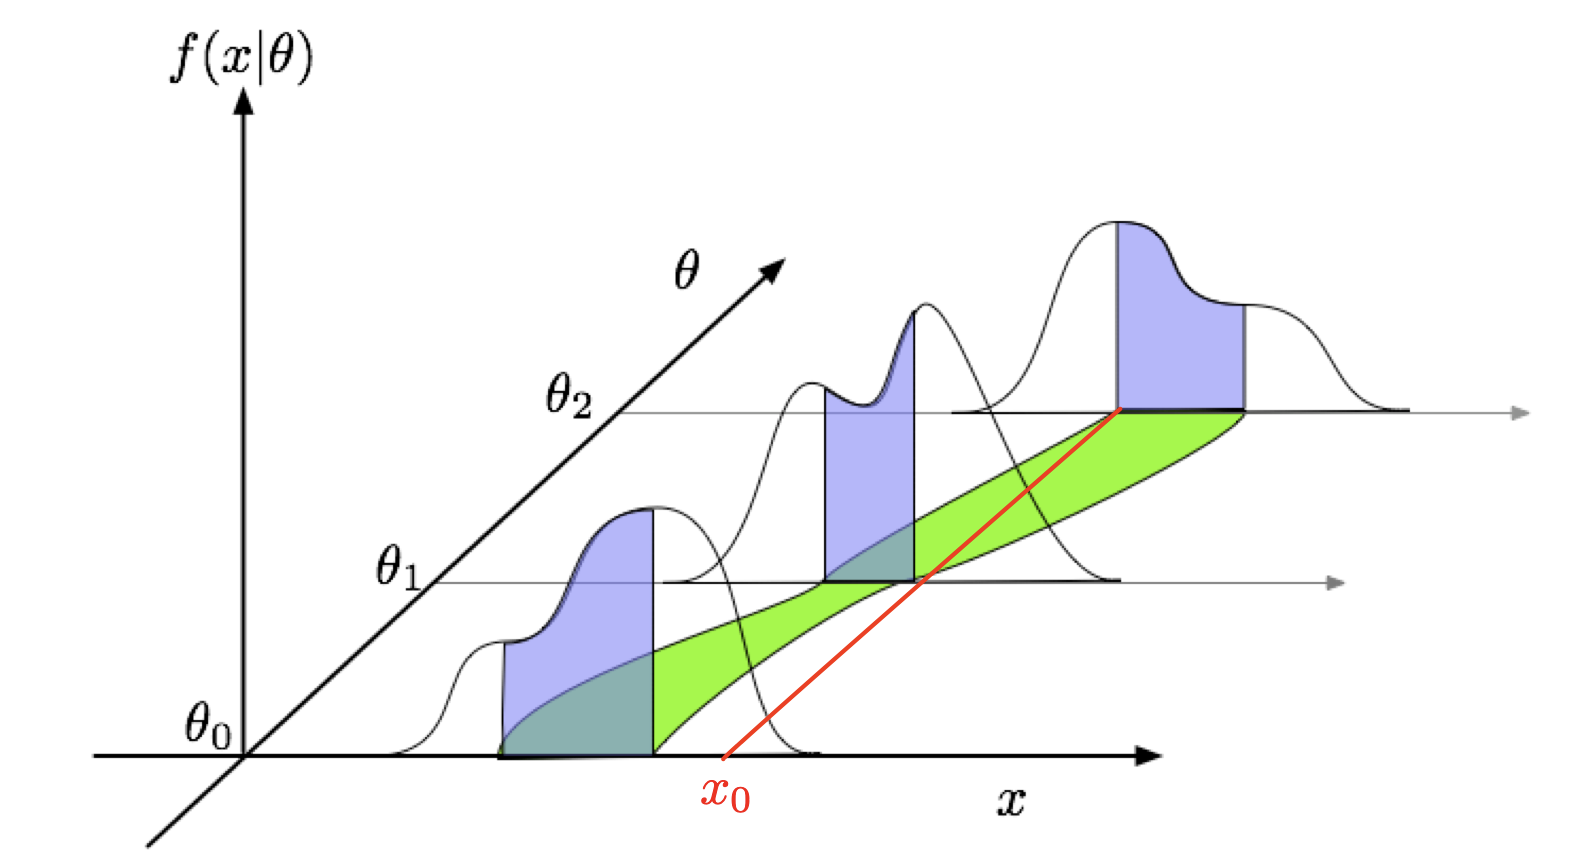
\includegraphics[width=12cm]{figures/ch-9-event-categorization-and-signal-extraction/schematic_neyman_construction.png}
    \caption[Schematic of the Neyman construction for confidence intervals.]{Schematic of the Neyman construction for confidence intervals~\cite{2011-Statistics-Cranmer}. For each value of $\theta$, we find a region in $x$ where $\int f(x|\theta) dx$ satisfies the size of the test (\textit{blue}). These regions form a confidence belt (\textit{green}). The intersection of the observation $x_0$ (\textit{red}) with the confidence belt defines the confidence interval $[\theta_1, \theta_2]$~\cite{2011-Statistics-Cranmer}.} 
    \label{fig:neyman-construction}
\end{figure}

\subsection{Profile likelihood ratio}

In this section we describe a frequentist statistical procedure based on the profile likelihood ratio test statistic, which is implemented using asymptotic distributions.

With a multi-parameter likelihood function $L(\boldsymbol{\alpha})$, the the maximum likelihood of one specific parameter $\alpha_p$ with other parameters $\boldsymbol{\alpha}_o$ fixed, is called the conditional maximum likelihood estimate and is denoted $\doublehat{\alpha}_p(\boldsymbol{\alpha_0})$.
The process of choosing specific values of the nuisance parameters for a given value of $\mu$, $\mathcal{D}_{\text{simulated}}$, and value of global observables $\mathcal{G}$ is called profiling. From the full list of parameters $\boldsymbol{\alpha}$, we denote the parameter of interest $\mu$, and the nuisance parameters $\boldsymbol{\theta}$.

We construct the profile likelihood ratio,
\begin{equation}
    \lambda(\mu) = \frac{L(\mu, \doublehat{\boldsymbol{\theta}}(\mu))}{L({\mu, \hat{\boldsymbol{\theta}}})}
\end{equation}
which depends explicitly on the parameter of interest $\mu$, implicitly on the data $\mathcal{D}_{\text{sim}}$ and global observables $\mathcal{G}$, and is independent of the nuisance parameters $\boldsymbol{\theta}$, which have been eliminated in profiling~\cite{2011-Statistics-Cranmer}.

The main conceptual reason for constructing the test statistic from the profile likelihood ratio is that asymptotically (i.e. for measurements with many events) the distribution of the profile likelihood ratio $\lambda(\mu = \mu_{\text{true}})$ is independent of the values of the nuisance parameters~\cite{2011-Statistics-Cranmer}. 

The following $p$-value is used to quantify the consistency with the hypothesis of a signal strength of $\mu$:
\begin{equation}
    p_\mu = \int_{\tilde{q}_{\mu, \text{obs}}}^{\infty} f(\tilde{q}_\mu | \mu, \doublehat{\boldsymbol{\theta}}(\mu, \text{obs})) \, d\tilde{q}_\mu
\end{equation}


\subsection{Modified frequentist method: \texorpdfstring{$CL_{S}$}{CLs}}
In the modified frequentist method called $CL_{S}$, to test a hypothesis with signal, we define $p'_{\mu}$ as a ratio of $p$-values~\cite{2011-Statistics-Cranmer}:
\begin{equation}
    p'_{\mu} = \frac{p_\mu}{1 - p_b}
\end{equation}
where $p_b$ is the $p$-value derived under the background-only hypothesis:
\begin{equation}
    p_b = 1 - p_0 \equiv 1 - \int_{\tilde{q}_{\mu, \text{obs}}}^{\infty} f(\tilde{q}_\mu | 0, \doublehat{\boldsymbol{\theta}}(\mu = 0, \text{obs})) \, d\tilde{q}_{\mu} \, .
\end{equation}
The $CL_{S}$ upper limit on $\mu$, denoted $\mu_{up}$, is obtained by solving for $p'_{\mu_{\text{up}}} = 5\%$. If testing the compatibility of the data with the background-only hypothesis, we consider the $p_b$ value defined above and conventionally convert it into the quantile or ``sigma" of a unit Gaussian. $z$ standard deviations (e.g. $z = 5$ in ``5$\sigma$") means that the probability of falling above these standard deviations, equals $p_b$ (e.g. $3\sigma$ corresponds to $p_b = 2.7 \times 10^{-3}$ or 95.43\%, and $5\sigma$ corresponds to $p_b = 5.7 \times 10^{-7}$ or 99.999943\%).
